

\documentclass[table,10pt]{beamer}
%%%%%%%%%%%%%%%%%%%%%%%%%%%%%%%%%%%%%%%%%%%%%%%%%%%%%%

%%%%%%%%%%%%%%%%%%%%%%%%%%%%%%%%%%%%%%%%%%%%%%%%%%%%%%%%%%%%%%%%
%%%%%%%%%%%%%%%%%%%%%%%%%%%%%%%%%%%%%%%%%%%%%%%%%%%%%%%%%%%%%%%%%%%%%%%%%%%%%%%%%%%%%%%%%%%%%%%%%%%%%%%%%%%%%%%%%%%%%%%%%%%%%%%%%%%%%%

\usepackage{hyperref}
\usepackage{pstricks,  epsf,psfrag,float}
\usepackage{multirow,hhline, epsfig,graphpap,pspicture,float}
\usepackage{subcaption}
\usepackage{colortbl}
\usepackage{amsmath}
\usepackage{threeparttable}
\usepackage{booktabs}
%\usepackage[absolute,overlay]{textpos}


\usetheme{Malmoe}

%%%%%%%%%%%%%%%%%%%%%%%%%%%%%%%%%%%%%%%%%%%%%%%%%%%%%%%%%%%%%%%%%%%%%%%%%%%%

\newenvironment{stepenumerate}{\begin{enumerate}[<+->]}{\end{enumerate}}
% \newenvironment{itemize}{\begin{itemize}[<+->]}{\end{itemize} }
\newenvironment{stepenumeratewithalert}{\begin{enumerate}[<+-| alert@+>]}{\end{enumerate}}
\newenvironment{itemizewithalert}{\begin{itemize}[<+-| alert@+>]}{\end{itemize} }

\useoutertheme{infolines}
\useinnertheme{rectangles}
\definecolor{link}{gray}{0.5}
\definecolor{uchile}{rgb}{0.13,0.13,0.44}
\definecolor{stern}{rgb}{0.34,0.02,0.55}
\definecolor{highlight}{rgb}{0.87,0.87,0.87}
\definecolor{cellhighlight}{rgb}{1.00,1.00,0.53}
\definecolor{dred}{rgb}{0.68,0.00,0.00}
\definecolor{darkgray}{gray}{0.75}
\definecolor{lgray}{rgb}{0.85,0.85,0.85}
\definecolor{yaleblue}{rgb}{0.0,0.28,0.57}
\definecolor{princeton}{rgb}{1.00,0.56,0.00}
%\textcolor[rgb]{0.47,0.00,0.00}{}
\setbeamercolor*{normal text}{fg=black,bg=white}
\setbeamercolor*{alerted text}{fg=princeton}
\setbeamercolor*{example text}{fg=stern}
\setbeamercolor*{structure}{fg=princeton}

\setbeamerfont{alerted text}{series=\bfseries}

\setbeamercolor{palette primary}{fg=black,bg=white}
\setbeamercolor{palette secondary}{fg=black,bg=princeton}
\setbeamercolor{palette tertiary}{fg=black,bg=white}
\setbeamercolor{palette quaternary}{fg=princeton,bg=black}

\setbeamercolor*{author in head/foot}{parent=palette quaternary}
\setbeamercolor*{title in head/foot}{parent=palette quaternary}
\setbeamercolor*{date in head/foot}{parent=palette quaternary}
\setbeamercolor*{section in head/foot}{parent=palette secondary}
\setbeamercolor*{subsection in head/foot}{parent=palette quaternary}
\setbeamercolor*{titlelike}{parent=palette tertiary}


\setbeamercovered{%
%still covered={\opaqueness<1>{20}\opaqueness<2>{10}\opaqueness<3>{5}\opaqueness<4->{2}},
again covered={\opaqueness<1->{100}}}
\setbeamertemplate{navigation symbols}{}

\ProcessOptionsBeamer
\newcommand{\rl}[1]{\addtolength{\extrarowheight}{#1mm }}

\newcommand{\semitransp}[2][35]{\color{fg!#1}#2}
\newcommand{\light}[1]{\textcolor{gray}{#1}}

%%%%%%%%%%%%%%%%%%%%%%%%%%%%%%%%%%%%
\title[College Major and Selectivity]{Student Choices and the Return to College Major and Selectivity}
     \author[Christopher A. Neilson]{\small{   \textbf{Christopher A. Neilson} \\ Princeton University \& NBER \\\vspace{.1in} \textbf{Justine Hastings }\\ Brown University \& NBER\\ \vspace{.1in} \textbf{Seth D. Zimmerman} \\ University of Chicago \& NBER} }
  %   \author[Christopher A. Neilson]{{ {Christopher A. Neilson}\\ Princeton University \& NBER  } }
\institute[Princeton University]{ }
\titlegraphic{\includegraphics[width=0.4\textwidth]{Figures/princeton_logo.eps}}
% \includegraphics[width=0.3\textwidth]{logo_mineduc.eps}
\date[Nov 2018]{Stanford GSB}




\begin{document}
\maketitle
%-----------------------------------------------------------------------
\section{Motivation}

% Earnings inequality (altonji et al review), determinantes of earnings inequality within college graduates (skills, talents, others)

% notoriously difficult to identify these effects given potential for unobservable talent and preferences




\begin{frame}{Motivation}

% Labor income for males 30-55

\begin{figure}
  \centering
  \includegraphics[width=0.85\textwidth]{Figures/distributionEarnings45.eps}

\end{figure}

\end{frame}

\begin{frame}{Motivation}

\begin{itemize}

\item<1> Altonji, Blom and Meghir (2012) document the large dispersion of earnings within college graduates. 
\bigskip


\item<2> Understanding the underlying causes is important for understanding inequality and designing policy/regulation in higher education.
\bigskip

\item<3> Higher education \alert{production function} and student \alert{preferences} is an input to studying many policy choices. 
\bigskip

\begin{itemize}
\item<4>[\alert{$\Rightarrow$}] Demand Side: Allocation of subsidies and loans, Information disclosure policies 
\smallskip 
\item<5>[\alert{$\Rightarrow$}] Supply Side: Minimal quality standards, Accountability policies and funding incentives
\end{itemize}


\end{itemize}
\end{frame}



\begin{frame}{Question }

\begin{itemize}

\item<2> Would like to answer questions such as:

\begin{itemize}
\item<2> If I move a student from degree $A$ to degree $B$, how would earnings change? \medskip
\item<2> How does this depend on attributes of degree, student?\medskip
\item<2> If I closed degree $A$ and made students go elsewhere, where would they go?
\end{itemize}

\medskip

\item<3> Several types of evidence available
\begin{itemize}
\item<3> OLS estimates $\rightarrow$ widely available, but not causal?
\medskip

\item<3> RD estimates $\rightarrow$ credibly causal, but only for some students/margins.
\medskip

\item<3> Mapping from people to programs  $\rightarrow$  tells us about selection, but not earnings.
\end{itemize}

\bigskip
\item<4> How do we aggregate this evidence? How can we use this to design policy and regulation?


\end{itemize}

\end{frame}



\begin{frame}
\frametitle{What we do}

\begin{itemize}
\item<1> \alert{Collect/Create Crazy Data} Obtain and digitalize centralized college applications/admissions for $\thicksim$ 40 cohorts of students and merge to tax records.
  
\item<2> \alert{New evidence} Present new ``reduced form'' evidence on
\begin{itemize}
\item<2> Heterogeneity in earnings effects of college by field of study and selectivity
\item<3> How field premia vary by student characteristics
\item<4> How OLS estimates compare to RD estimates
\end{itemize}

\medskip

\item<5> Show how to link OLS and RD estimates in same framework

\begin{itemize}
\item<6> Develop a model of college major choice and a earnings determination that allow us to knit together many RD, OLS estimates
\item<7> $\rightarrow$ Recover distribution of treatment effects
\end{itemize}

\medskip

\item<8> Using estimated model:

\begin{itemize}
\item<9> \alert{Quantify earnings differentials}  by majors, by course content, by selectivity.\\ \medskip

\item<10> \alert{Decompose earnings} into homogeneous/heterogeneous and observable/unobservable characteristics.\\
\medskip

\item<11> \alert{Evaluate Policy} Evaluate policies simulate counterfactual ``accountability'' policies. What if we shut down low-earning degrees?
\end{itemize}

\end{itemize}

\end{frame}




%
%\begin{frame}{What we do}
%
%Specifically we conduct the following empirical exercises:
%\medskip
%
%\begin{enumerate}
%  \item<2> \alert{Get/Create Crazy Data} Obtain nd digitalize college applications, characteristics and merge to tax records for $\thicksim$ 40 cohorts of students.
%  \medskip
%  \begin{itemize}
%  \item<3> $\rightarrow$ New dataset replicating one of the oldest centralized assignment mechanisms for higher education linked to administrative records.
%  \end{itemize}
%
%  \item<4> \alert{Estimate OLS} for life cycle income conditional on test scores, gender, SES, and degree study.
%  \medskip
%  \begin{itemize}
%  \item<5> $\rightarrow$ New reduced form evidence on determinants of lifetime earnings based on major and college characteristics.
%  \end{itemize}
%
%  \item<6> \alert{Estimate RDs} Using administrative data on centralized college applications and results we estimate RD across over thousands of margins.
%
%  \begin{itemize}
%  \item<7> $\rightarrow$ New reduced form evidence on heterogeneous treatment effects of attending different majors and universities for marginal candidates.
%  \end{itemize}
%  \medskip
%
%  \item<8> \alert{Estimate Model} Develop empirical model of selection and earnings determination to knit together many RD, OLS estimates
%  \begin{itemize}
%  \item<9> $\rightarrow$ Recover distribution of treatment effects.
%  \item<10> $\rightarrow$ Conduct policy analysis.
%
%  \end{itemize}
%
%\end{enumerate}
%
%
%\end{frame}

%
%\begin{frame}{Quick overview}
%
%\begin{itemize}
%  \item<1> The context and data under study is the population of Chilean college graduates entering higher education between 1967 and 2003.
%  \medskip
%
%  \item<2> Model college/major choices and income jointly with the potential for classic self selection.\medskip
%\medskip
%
%  \item<3> To estimate model, we leverage unique administrative data and institutional features from the Chilean system that will provide variation across a large set of margins.
%  \medskip
%
%\begin{enumerate}
%  \item Take advantage of centralized admissions system. \smallskip
%
%  \item Test scores, application lists, admissions outcomes for participants. \smallskip
%
%  \item Decomposition of all higher education options into course content, institution and level of selectivity.  \smallskip
%
%  \item Link this data to administrative data on a decade of current tax income.
%\end{enumerate}
%
%
%\end{itemize}
%\end{frame}
%


\section{Data Sources and Structure}\subsection{Data}


\begin{frame}{Data Sources and Structure} % two slides
\centering

\begin{itemize}
  \item<1> The context is the population of Chilean college graduates entering higher education between 1967 and 2003.
  \medskip

  \item<2> The system has used centralized admissions and an set of entrance exams since the late 1960s and until the early 1990s included all college options.
    \medskip

  \item<3> Data is created by huge 7 year digitalization process; over 40 million keystrokes.
    \medskip

  \item<4> Work closely with several government agencies including the local tax authority. % as well as Ministry of Labor, Testing Agencies, Ministry of Education, Civil Registry).
      \medskip

   \item<5> Several practical limitations regarding data use and access influence the empirical strategy chosen.
    \medskip

\end{itemize}


\end{frame}


\begin{frame}{Data Sources and Structure} % two slides
\centering

\begin{itemize}

\item<2-3> \alert{Test Scores and GPA (PAA)} 1967-2003. This includes scores, GPA, gender, and high school of all test takers.\medskip
\only<2>{
\centering

\includegraphics[width=0.7\textwidth]{Figures/admision_1977.eps}%
}

\only<3>{
\includegraphics[width=0.7\textwidth]{Figures/Antecedentes_Example.eps}%
}


\item<4> \alert{Full College Applications} 1976-1988 and 2000-2003. This includes the full application list and the condition of the application, whether it be admitted, waitlisted or not valid.\medskip

\only<4>{
\includegraphics[width=0.43\textwidth]{Figures/takingPicturesBooks.eps}$\quad$
\includegraphics[width=0.43\textwidth]{Figures/booksDEMRE.eps}%
}

\item<5>  \alert{College Application Results} 1976-2003. This includes the admitted and wait listed applications.\medskip

\item<6>  \alert{Earnings} 2006-2016.  Decade of earnings data from the tax agency.\medskip
%
\item<7>  \alert{College Major Course Content.} Data by educational option regarding semesters of STEM, professional training, etc.  \medskip
\end{itemize}



\end{frame}

%\begin{frame}
%\centering
%
%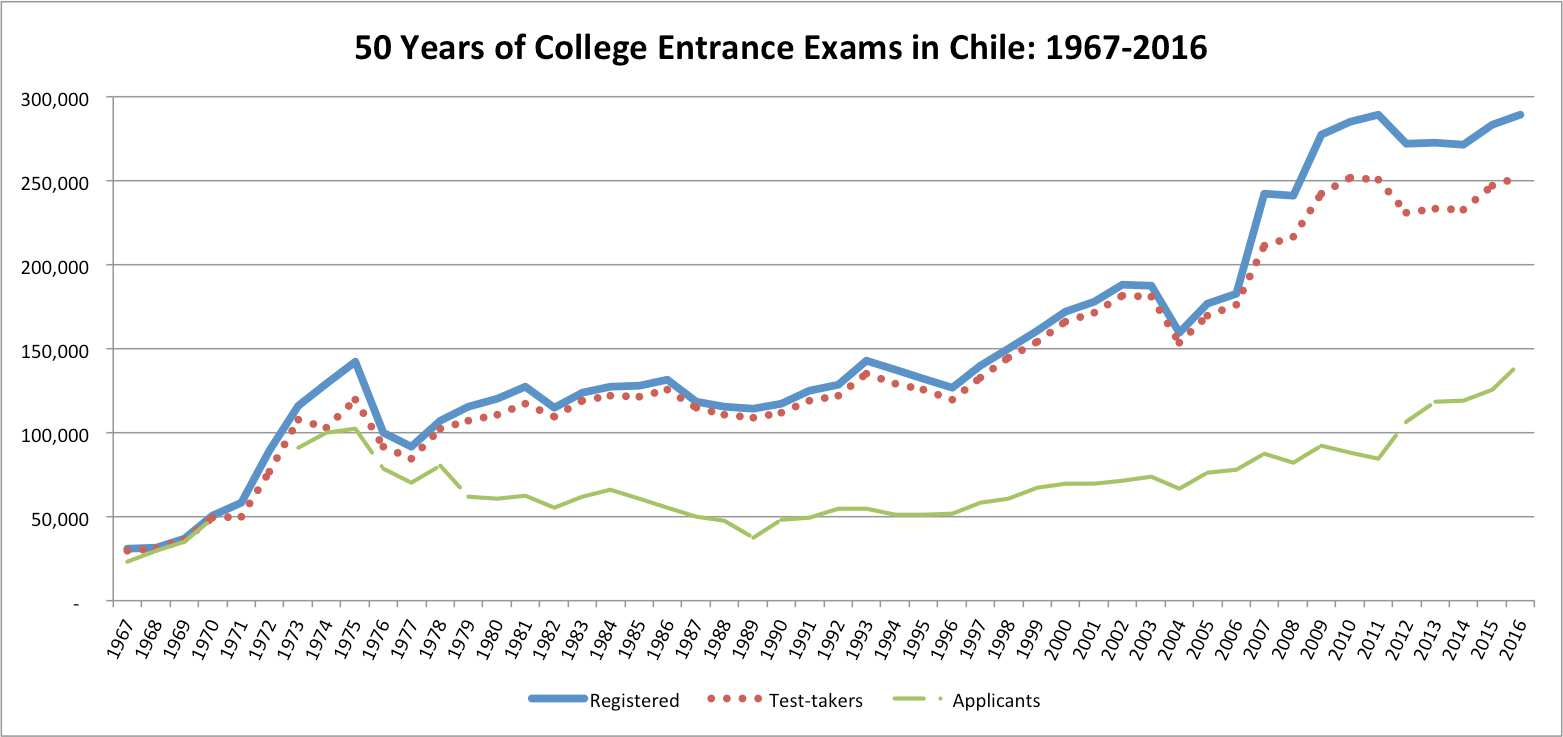
\includegraphics[width=0.9\textwidth]{Figures/50years.eps}%
%
%\end{frame}





%
%\begin{frame}
%  \centering
%\only<1>{
%  \includegraphics[width=\textwidth]{Figures/ApplicationDescriptive.eps}%
%  }
%%  \only<2>{
%%  \includegraphics[width=0.7\textwidth]{Figures/ProbApplication.eps}%
%%  }
%%
%\end{frame}


\frame{
\frametitle{Distribution of target and next option degree programs}

\begin{scriptsize}

\begin{table}[htbp]\centering
\caption{\label{Target area by next year}}
\textbf{Target area by next area \% terms }
\begin{tabular} {@{} l r  r  r  r  r  r  r  r  r  r r @{}} \\ \hline
& \multicolumn{11}{@{} c @{}}{\textbf{$j^{a+1}$ Area}} \\
\textbf{$j^a$ Area} &
           Bus  &Ag &Art & Sci &Soc & Law&Educ &Hum &Hth &Tech &all \\  \hline
Business &    \cellcolor{gray} 49.5&      6.3&      1.7&      4.3&      4.7&      0.7&      6.0&      1.3&      0.5&  \cellcolor{princeton}   25.2&    100.0\\
Agriculture &      5.6&   \cellcolor{gray}  50.3&      1.5&      5.7&      2.2&      0.6&      6.5&      0.4&      3.6&  \cellcolor{princeton}   23.5&    100.0\\
Art \& Arch&      4.6&      3.5&   \cellcolor{gray}  49.7&      2.2&      6.1&      1.4&      7.3&      2.2&      0.5&   \cellcolor{princeton}  22.4&    100.0\\
Basic Science &      5.1&      9.9&      1.9&  \cellcolor{gray}   24.7&      4.8&      0.6&     12.4&      1.1&      9.1&  \cellcolor{princeton}   30.3&    100.0\\
Social Science &      8.3&      3.9&      4.8&      4.2&   \cellcolor{gray}  39.6&      6.3&   \cellcolor{princeton}  14.0&      6.0&      2.7&     10.3&    100.0\\
Law&      5.9&      2.1&      2.1&      1.3&   \cellcolor{princeton}  21.5&  \cellcolor{gray}   50.7&      6.0&      3.7&      2.0&      4.7&    100.0\\
Education &    4.8&      5.2&      2.3&      5.1&      5.0&      0.9&   \cellcolor{gray}  59.1&      4.3&      1.2&     12.1&    100.0\\
Humanities&      5.2&      2.6&      6.6&      2.4&     11.7&      3.0&   \cellcolor{princeton}  28.5&    \cellcolor{gray} 34.1&      0.2&      5.5&    100.0\\
Health&      1.4&      5.5&      0.9&   \cellcolor{princeton}   9.3&      3.8&      1.4&      4.3&      0.5&    \cellcolor{gray} 63.6&      9.4&    100.0\\
Technology&    \cellcolor{princeton}  8.6&      7.6&      1.9&      5.8&      1.3&      0.2&      4.0&      0.7&      1.9&  \cellcolor{gray}   67.8&    100.0\\
Total&     10.9&      9.7&      4.8&      6.3&      7.2&      3.7&     12.8&      2.5&      9.1&     33.1&    100.0\\\hline
\end{tabular}
\end{table}
\end{scriptsize}

}


%\frame{
%\frametitle{Distribution of target and next option degree programs}
%
%\begin{scriptsize}
%
%\begin{table}[htbp]\centering
%\caption{\label{distsel}
%\textbf{Target tercile by Next tercile~(\%)}}
%\begin{tabular} {@{} l r  r  r r @{}} \\ \hline
%& \multicolumn{4}{@{} c @{}}{\textbf{Next tercile}} \\
%\textbf{Target tercile} &
%Lowest &Middle &Highest &Total \\  \hline
%Lowest&     82.2&     17.6&      0.2&    100.0\\
%Middle&     19.5&     65.1&     15.4&    100.0\\
%Highest&      0.7&     13.9&     85.4&    100.0\\
%Total&     30.3&     33.0&     36.8&    100.0\\\hline
%\end{tabular}
%\end{table}
%
%\end{scriptsize}
%
%}





\begin{frame}{Describing Types of Higher Education}
\centering


\only<1>{
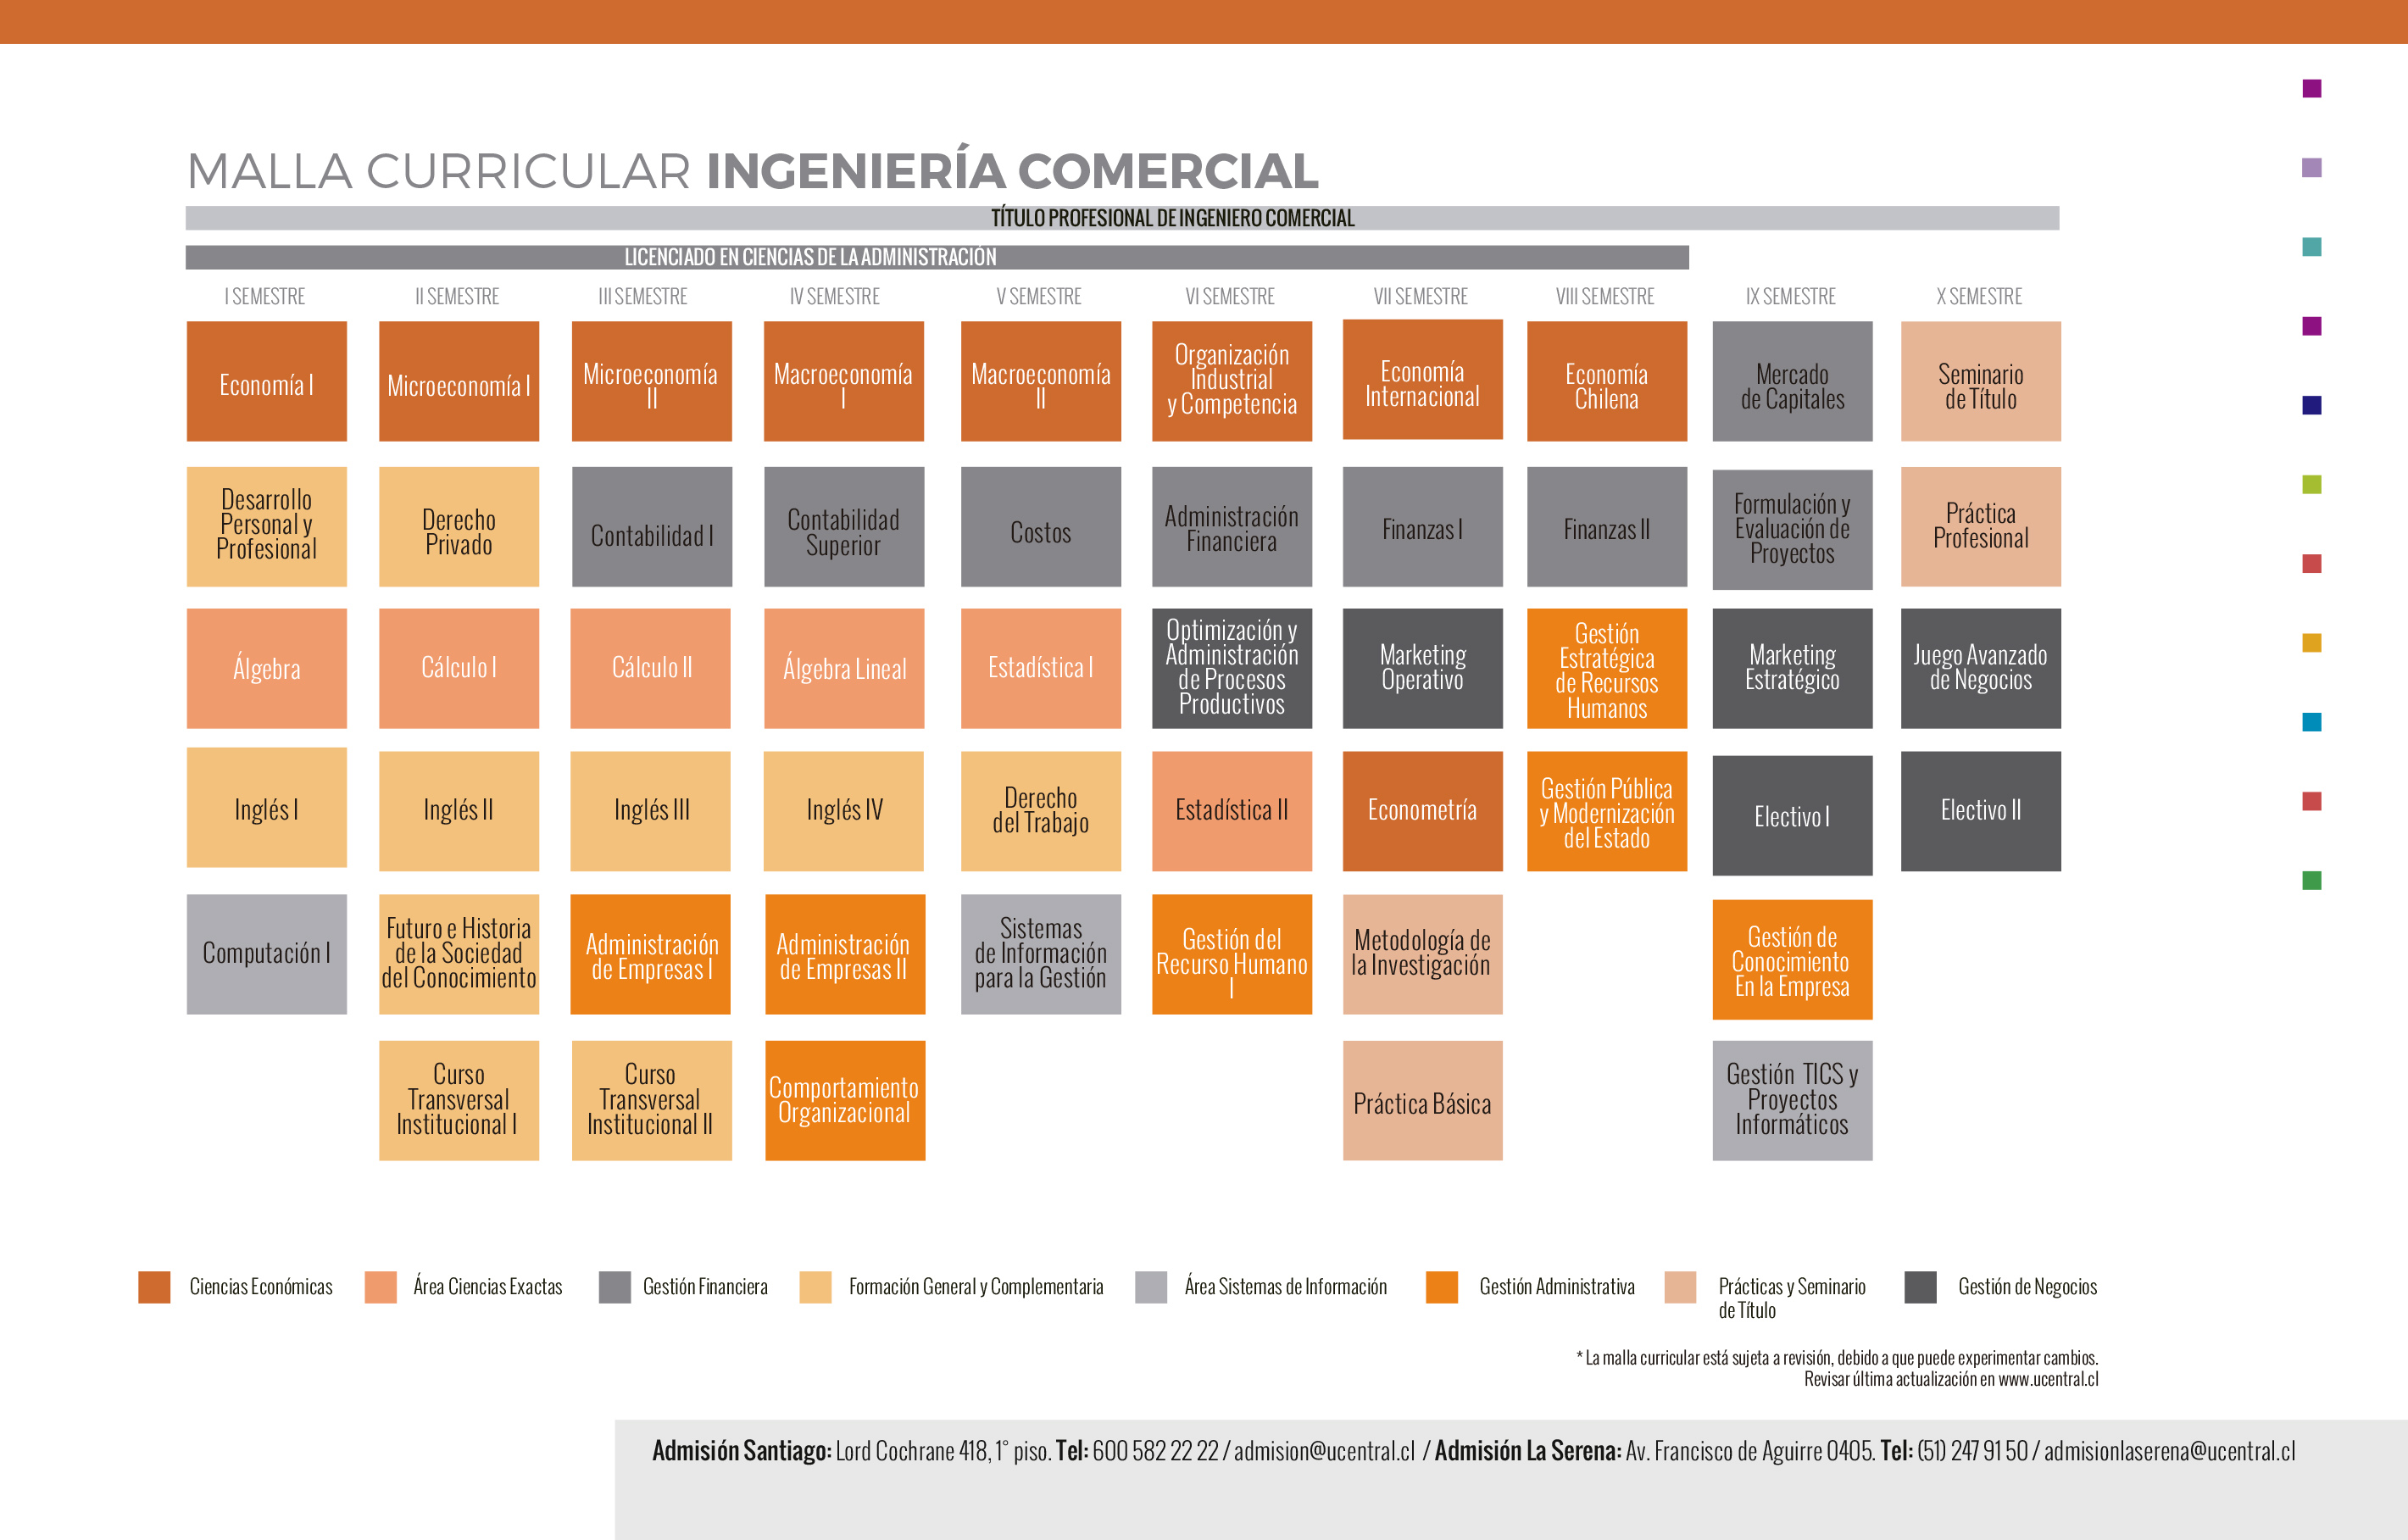
\includegraphics[width=0.95\textwidth]{Figures/foto_malla1.eps}%
}

\only<2>{
\includegraphics[width=0.95\textwidth]{Figures/foto_malla2.eps}%
}



\end{frame}



\frame{
\frametitle{Share of Course Content over Categories}


\begin{table}[htbp]\centering
\caption{\label{}
\textbf{Course Composition Share by Field} }
\begin{tabular} {l r r r} \\
\hline\textbf{Target Area } & \textbf{ STEM} & \textbf{ Professional} & \textbf{  Qualitative} \\
\hline
Basic Science      & 0.621 & 0.217 & 0.163 \\
Health             & 0.553 & 0.239 & 0.208 \\
Agriculture        & 0.546 & 0.306 & 0.148 \\
Business           & 0.562 & 0.215 & 0.222 \\
Technology         & 0.508 & 0.295 & 0.197 \\
Art y Architecture & 0.206 & 0.194 & 0.600 \\
Law                & 0.209 & 0.168 & 0.623 \\
Social Science     & 0.175 & 0.220 & 0.604 \\
Humanities         & 0.178 & 0.183 & 0.639 \\
Education          & 0.158 & 0.196 & 0.646 \\

Overall            & 0.420 & 0.246 & 0.333 \\
\hline
\end{tabular}
\end{table}


}
%
%\begin{frame}{STEM share and selectivity}
%\begin{table}[htbp]\centering
%\caption{\label{}
%\textbf{Credits by Selectivity } }\begin{tabular} {@{} l r r r @{}} \\ \hline\textbf{Selectivity Tercile} & \textbf{STEM} & \textbf{ Professional} & \textbf{Qualitative} \\
%\hline
%Lowest  	&0.40	&0.26	&0.34\\
%Middle  	&0.41	&0.24	&0.35\\
%Highest  	&0.45	&0.24	&0.31\\ \hline
%			&       &       &    \\
%Total  	    &0.42	&0.25	&0.34\\
%\hline
%\end{tabular}
%\end{table}
%\end{frame}
%
%



\subsection{Earnings and Test Scores}
\begin{frame}{Empirical Fact 1 : Steep Test Score Gradient }
\centering

\begin{figure}
  \centering
  \includegraphics[width=0.6\textwidth]{Figures/earnings_by_score.eps}

\end{figure}

\end{frame}
\begin{frame}{Empirical Fact 2 : Steep Test Score Gradient to Math }
\centering

\begin{figure}
  \centering
  \includegraphics[width=0.9\textwidth]{Figures/earnings_math_lang.eps}

\end{figure}

\end{frame}



\subsection{Earnings and Fields of Study}

\begin{frame}{Empirical Fact 3 : Heterogeneity by Area/Major  }

\centering
\begin{figure}
  \centering
  \includegraphics[width=0.8\textwidth]{Figures/earnings_area.eps}

\end{figure}
\end{frame}

\begin{frame}
\frametitle{OLS specifications}

OLS specifications:
\begin{align}
Y_{ijt}&=X_{it} \Gamma+v_{ijt} \\
v_{ijt}&=\widetilde{\varphi}_{j}+e_{ijt} \nonumber
\end{align}
\vspace{-.2in}
\begin{itemize}
\item <1> Step 1: Estimate $\hat{\Gamma}$
\item<1> Step 2: using $\hat{\Gamma}$, compute mean degree-specific residuals $\overline{v}_{j}$
\item<1> Step 3: shrink $\overline{v}_{j}$ back towards zero to obtain best predictors $\widehat{\widetilde{\varphi}}_j$.
\item<1> Controls: math scores, reading scores, gender, HS type (SES), GPA
\end{itemize}

\medskip

Look at unweighted distribution of effect estimates, mean normalized to zero
\end{frame}


%\begin{frame}{Empirical Fact 3 : Heterogeneity of Area/Major Effects}
%\begin{center}
%\begin{minipage}[f]{\textwidth}
%\begin{figure}[H]
% \centering
%\vspace{-.1in}
%\includegraphics[width=.8\textwidth]{Figures/OLS_g1.png}
%\end{figure}
%\end{minipage}
%\end{center}
%\end{frame}


\begin{frame}{Empirical Fact 3 : Heterogeneity of Degree Effects   }
	\begin{center}
		\includegraphics[height=.8\textheight]{Figures/FL-FE-byarea.pdf}
	\end{center}
\end{frame}


\begin{frame}{Empirical Fact 4 : Heterogeneity by Degree Characteristics }
\textbf{OLS Estimates of Biased FE $\widetilde{\varphi_j}$ by course content}
\begin{center}
\begin{figure}[H]
\centering
\begin{subfigure}{0.5\textwidth}
\centering
    \includegraphics[width=\linewidth]{Figures/FL-FE-byCquant_q3.pdf}
    \caption{By number of STEM semester credits}
\end{subfigure}%
\begin{subfigure}{0.5\textwidth}
\centering
    \includegraphics[width=\linewidth]{Figures/FL-FE-byPquant_q3.pdf}
    \caption{By share of STEM semester credits}
\end{subfigure}
\end{figure}
\end{center}
\end{frame}

\begin{frame}{Empirical Fact 4 : Heterogeneity by Degree Characteristics }
\begin{center}
\textbf{OLS Estimates of Biased FE $\widetilde{\varphi_j}$ by course content even Within Broad Area}
\begin{figure}[H]
\centering
\begin{subfigure}{0.5\textwidth}
\centering
    \includegraphics[width=\linewidth]{Figures/FL-FE-byCquant_q2-Area2.pdf}
    \caption{Agriculture}
\end{subfigure}%
\begin{subfigure}{0.5\textwidth}
\centering
    \includegraphics[width=\linewidth]{Figures/FL-FE-byCquant_q2-Area11.pdf}
    \caption{Technology}
\end{subfigure}
\end{figure}
\end{center}
\end{frame}


\begin{frame}{Empirical Fact 4 : Heterogeneity by Degree Characteristics }


\centering
\only<1>{
\textbf{FE projected on Quant Courses }

\includegraphics[width=1.1\textwidth]{Figures/StemFE.eps}
  }


  \only<2>{

\textbf{FE projected on Quanl Courses }
\includegraphics[width=1.1\textwidth]{Figures/QualiFE.eps}
  }


  \only<3>{
\textbf{Distribution of FE by Selectivity Tercile }
\includegraphics[width=.8\textwidth]{figures/OLS_g1b.png}
  }

\end{frame}


%\begin{frame}{Empirical Fact 4 : Heterogeneity by Degree Characteristics }
%
%\begin{center}
%\begin{itemize}
%\item<1> Field: e.g., Tech high, Art low)
%\item<2> Selectivity: higher sel $\rightarrow$ higher earnings
%\item<3> Course content: more quant $\rightarrow$ higher earnings; reverse for qual
%\end{itemize}
%\begin{minipage}[f]{\textwidth}
%\begin{figure}[H]
% \centering
% \only<1>{
%\includegraphics[width=.6\textwidth]{figures/OLS_g1a.png}
%}
%\only<2>{
%\includegraphics[width=.6\textwidth]{figures/OLS_g1b.png}
%}
%\only<3>{
%\includegraphics[width=.6\textwidth]{figures/OLS_g1c.png}
%}
%\only<4>{
%\includegraphics[width=.6\textwidth]{Figures/OLS_g1d.png}
%}
%\end{figure}
%\end{minipage}
%\end{center}
%\end{frame}



\begin{frame}{Empirical Fact 4 : Heterogeneity by Some Match Effects }


\begin{center}
\begin{scriptsize}
\input{Figures/OLS_chars1_a}
\end{scriptsize}
\end{center}
\end{frame}

\begin{frame}{Empirical Fact 4 : Heterogeneity by Some Match Effects }

%[input returns to scores ]
\begin{center}
\textbf{OLS regression on broad areas by subgroup (Omitting Technology)}
\begin{tiny}
\only<1>{
\input{Figures/OLS_chars3_a.tex}
}
\only<2>{
\input{Figures/OLS_chars3_b.tex}
}
\end{tiny}
\end{center}
\end{frame}

\begin{frame}{Summary so far }

\begin{enumerate}
  \item<1> Heterogeneity by Student Score, especially math
  \item<2> Heterogeneity by Area/Major
  \item<3> Heterogeneity by Degree Characteristics, especially STEM and Selectivity
  \item<4> Match Effects
\end{enumerate}

\end{frame}



\begin{frame}{RD specifications provide new evidence}


Estimate RD specifications of the form

$$
Y_{ij}=\beta_0+\beta_1 A_{ij}+f(d_{ij})+e_{ijk}
$$
\begin{itemize}
\item $Y_{ijk}$ is income for student $i$ applying to degree $j$
\item $A_{ij}$ is admissions dummy, $f()$ is smooth function of $d_{ij}$.
\end{itemize}

\medskip

Split sample in several ways:
\begin{enumerate}
\item Quantiles of distribution of $\hat{\varphi}_j-\hat{\varphi}_k$, where $k$ is student $i's$ next option
\item Area of target degree $j$ and next in option $k$
\item Quantiles of distribution of $x_j-x_k$, for observable degree attribute $x_j$ such as course content
\end{enumerate}




\end{frame}


\begin{frame}{RD Case study: gains from admission to Tech degrees}
\begin{itemize}
\item Limited return to getting into Tech vs. next best thing
\item But that is because next best thing usually is also tech!
\item Subset on non-Tech $\rightarrow$ 10\% gain; Science only $\rightarrow$ 21\%
\end{itemize}
\centering
%[input returns to scores ]
\begin{center}
\begin{minipage}[f]{\textwidth}
\begin{figure}[H]
 \centering
\vspace{-.1in}
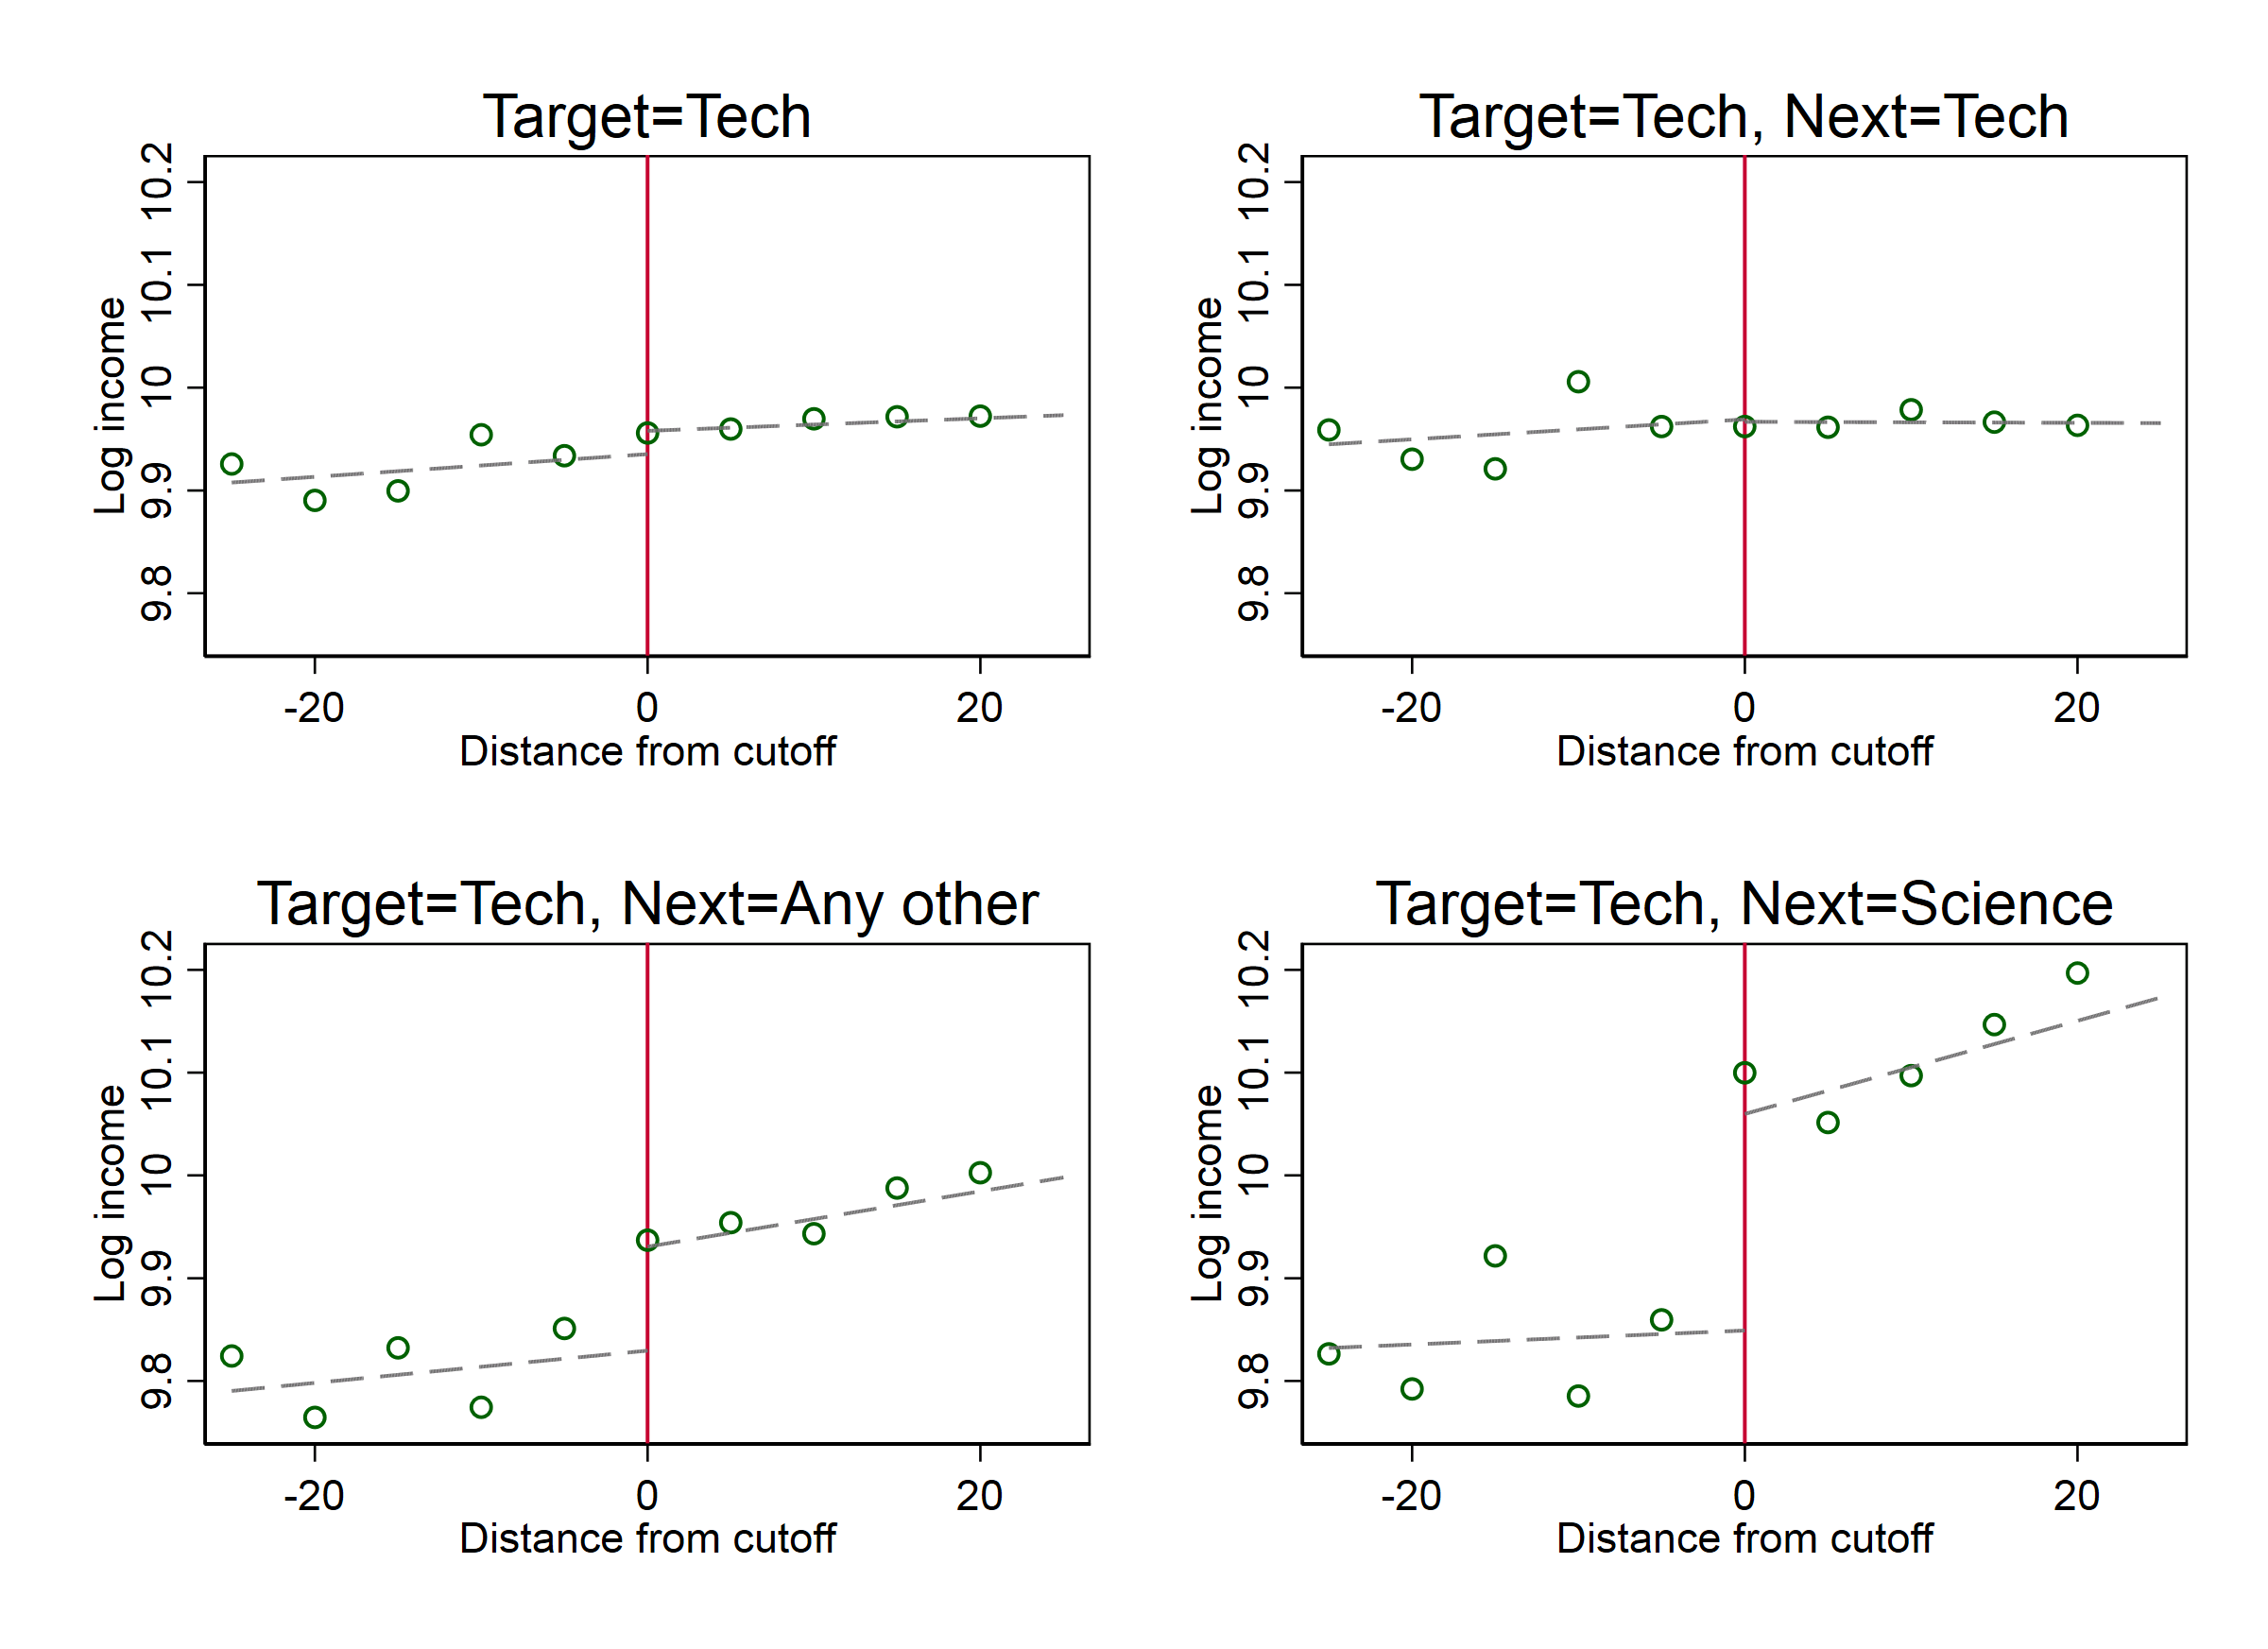
\includegraphics[width=.65\textwidth]{Figures/RD_gcomb.png}
\end{figure}
\end{minipage}
\end{center}
\begin{itemize}
\item<2> Have a lot of estimates like this!
\end{itemize}
\end{frame}



\begin{frame}{Empirical Fact 5 : What and where you study matter}

\textbf{RDs grouped by OLS prediction}
\begin{center}
\begin{figure}[H]
\includegraphics[width=.7\textwidth]{Figures/HighLowRDs.eps}
\end{figure}
\end{center}
\end{frame}

%\begin{frame}{RD effect by quartiles of OLS Prediction of Effect }
%    \begin{figure}
%    	\captionsetup[sub]{font=scriptsize,labelfont=scriptsize,belowskip=6pt,aboveskip=0pt}
%        \centering
%        \begin{subfigure}[b]{0.4\textwidth}
%            \centering
%            \includegraphics[width=\textwidth]{Figures/RDplot-tAreaXsnArea_q1.pdf}
%           	\caption{Quartile 1}
%        \end{subfigure}
%        \qquad
%        \begin{subfigure}[b]{0.4\textwidth}
%            \centering
%            \includegraphics[width=\textwidth]{Figures/RDplot-tAreaXsnArea_q2.pdf}
%            \caption{Quartile 2}
%        \end{subfigure}
%        \vskip\baselineskip
%        \begin{subfigure}[b]{0.4\textwidth}
%            \centering
%            \includegraphics[width=\textwidth]{Figures/RDplot-tAreaXsnArea_q3.pdf}
%            \caption{Quartile 3}
%        \end{subfigure}
%        \qquad
%        \begin{subfigure}[b]{0.4\textwidth}
%            \centering
%            \includegraphics[width=\textwidth]{Figures/RDplot-tAreaXsnArea_q4.pdf}
%            \caption{Quartile 4}
%        \end{subfigure}
%    \end{figure}
%\end{frame}
%
%
%
%\frame{
%\frametitle{RD by OLS prediction}
%\begin{center}
%\begin{figure}[H]
%\includegraphics[width=.8\textwidth]{Figures/OLS-RD-prediction.pdf}
%\end{figure}
%\end{center}
%
%}
%
%
%\begin{frame}{Empirical Fact 6 : OLS correlated with RD estimates}
%
%\begin{center}
%\begin{minipage}[f]{\textwidth}
%\begin{figure}[H]
% \centering
%\includegraphics[width=.6\textwidth]{figures/RD_g7b.png}
%\end{figure}
%\end{minipage}
%\end{center}
%\end{frame}



\begin{frame}{Empirical Fact 6 : OLS correlated with RD estimates}

\begin{center}
\begin{minipage}[f]{\textwidth}
\begin{figure}[H]
 \centering
\includegraphics[width=.6\textwidth]{figures/RD_g7a.png}
\end{figure}
\end{minipage}
\end{center}
\end{frame}

\begin{frame}{Empirical Fact 6 : OLS estimates correlated with RD}
\begin{itemize}
\item Compare RD to OLS  by area
\end{itemize}
\begin{center}
\begin{minipage}[f]{\textwidth}
\begin{figure}[H]
 \centering
\vspace{-.1in}
\includegraphics[width=.8\textwidth]{figures/RD_gArea.png}
\end{figure}
\end{minipage}
\end{center}

\end{frame}



\begin{frame}{Empirical Fact 7: Descriptive relationships do not always hold in RD}

\begin{itemize}
\item Quant does
\item Negative relationship w/ qual goes away
\item Positive relationship with selectivity goes away
\end{itemize}
\begin{center}
\begin{minipage}[f]{\textwidth}
\begin{figure}[H]
 \centering
\includegraphics[width=.6\textwidth]{figures/RD_DeltaQuant.png}
\end{figure}
\end{minipage}
\end{center}
\end{frame}


\begin{frame}{Empirical Fact 7: Descriptive relationships do not always hold in RD}

\begin{itemize}
\item Quant does
\item Negative relationship w/ qual goes away
\item Positive relationship with selectivity goes away
\end{itemize}
\begin{center}
\begin{minipage}[f]{\textwidth}
\begin{figure}[H]
 \centering
\includegraphics[width=.6\textwidth]{figures/RD_DeltaQual.png}
\end{figure}
\end{minipage}
\end{center}
\end{frame}



\begin{frame}{Empirical Fact 7: Descriptive relationships do not always hold in RD}

\begin{itemize}
\item Quant does
\item Negative relationship w/ qual goes away
\item Positive relationship with selectivity goes away
\end{itemize}
\begin{center}
\begin{minipage}[f]{\textwidth}
\begin{figure}[H]
 \centering
\includegraphics[width=.6\textwidth]{figures/RD_DeltaSel.png}
\end{figure}
\end{minipage}
\end{center}
\end{frame}


\begin{frame}{RD summary tables}

%[input returns to scores ]
\begin{center}
\begin{scriptsize}
\input{figures/RD_chars2a.tex}
\end{scriptsize}
\end{center}
\end{frame}
%
%
%
%\begin{frame}{Empirical Fact 7: OLS effects are heterogeneous by observables}
%\begin{itemize}
%\item Split sample by different binary variables
%\item Estimate OLS specifications separately within each sample
%\item Display correlation matrix of degree effect estimates for each group
%\end{itemize}
%
%\begin{center}
%\begin{scriptsize}
%\begin{tabular}{l cccc cccc}
%\input{figures/corrtab.tex}
%\end{tabular}
%\end{scriptsize}
%\end{center}
%\end{frame}
%
%

\begin{frame}{Empirical Fact 7: Heterogeneous effects predict RD estimates}


\begin{itemize}
\item<1>  Run RD specifications that allow for continuous interactions between admission, own-group predicted gains, and other-group predicted gains
$$
Y_{ij}=\beta_0+\beta_1A_{ij}+\beta_2  A_{ij}   \hat{\triangle}_{own}^{j,k} +\beta_3  A_{ij}  \hat{\triangle}_{other}^{j,k}+f(d_i,\hat{\triangle}_{own}^{j,k}, \hat{\triangle}_{other}^{j,k})+e_{ij}
$$
\item<1> Also allow for linear interactions between own- and other-group gains and polynomial terms
\item<1> All effects load on \emph{own} predictions, not others.
\end{itemize}

\uncover<2>{
\begin{center}
\begin{scriptsize}
\input{figures/rd_OLS_weights.tex}
\end{scriptsize}
\end{center}
}
\end{frame}







\begin{frame}{Empirical Fact 8: Selection associated with higher own-group effects}

\begin{itemize}
\item Look at sample of students admitted to each degree program $j$
\item Estimate  $Female_i=\beta_0+\beta_1 \hat{\varphi}_{female}^{j}+\beta_2 \hat{\varphi}_{all}^{j}+X_i \beta_3+e_i$, repeat for High SES.

\uncover<2>{
%[input returns to scores ]
\begin{center}
\begin{minipage}[f]{\textwidth}
\begin{figure}[H]
 \centering
\vspace{-.1in}
\includegraphics[width=.8\textwidth]{figures/RD_g8.png}
\end{figure}
\end{minipage}
\end{center}

\item Women and high SES show up more in degrees where own earnings higher
\item More women in degrees w/ low earnings overall, reverse for high-SES
}
\end{itemize}

\end{frame}


\begin{frame}{Taking Stock}

\begin{itemize}
  \item From OLS Evidence

\begin{enumerate}
  \item<1> Heterogeneity by Student Score, especially math
  \item<1> Heterogeneity by Area/Major
  \item<1> Heterogeneity by Degree Characteristics, especially STEM and Selectivity
  \item<1> Match Effects
\end{enumerate}

\item From RD Evidence
\begin{enumerate}
  \item<1> Evidence of heterogeneity in earnings effects across options in OLS also survives in RD setting, especially quant. 
   
  \item<2> Heterogeneity is correlated with student and option characteristics as well as interactions (course content,selectivity) 
  
  \item<3> Evidence of selection towards higher predicted earning options.
  
  \item<4> OLS and RD estimates are quite correlated.  
\end{enumerate}

\item<5> How to interpret this evidence in a systematic way? How to use it to inform policy? 

\end{itemize}
\end{frame}

% Simple model
\section{Model}
\subsection{Model of College Choice and Earnings}
\begin{frame}{Model of Preferences and Earnings}


\uncover<2>{\alert{Students}:

Let a student $i$ be characterized by $\left(x_i,{loc}_i,\psi,\tau,{\epsilon_i}\right)$. \medskip
\begin{tabular}{ll}
 $loc_i$:& location of students home. \\
 $x_i$:  &student entrance exam scores, SES and gender.\\
 $\psi_i$: & preference for educational options given its characteristics.\\
 $\tau_i$: & earnings ability if studying educational option given its characteristics.\\
$\epsilon_i$ : &  idiosyncratic preferences.
\end{tabular}
}

\medskip
\uncover<3>{\alert{Educational Options}:

Let educational options $j$ be characterized by $\left(x_j,{loc}_j, xc_j,\phi_j\right)$ \medskip
\begin{tabular}{ll}
 $loc_j$:& location of campus. \\
 $x_j$:  & institution, major characteristics including course content $c_j$ \\
 $c_j$ : & course content such as STEM, professional training, etc. \\
 $\varphi_j$: & additional value beyond course content.\\
\end{tabular}
}


\end{frame}

\begin{frame}{Simple Framework}

\uncover<1>{
\alert{Preferences :}
\begin{equation}\label{equ:utility}
u_{ij} = x_{j}\overline{\beta} + \beta^w f(w^e_{ij}) + \lambda D_{ij} + \psi_{ij} + \epsilon_{ij}
\end{equation}
}
\medskip

\uncover<2>{
\begin{equation}\label{equ:earnings}
\psi_{ij}= \sum_{k} x_{i}^k c_{j}^k \psi_k^o  +  c_j\psi^{u}_i
\end{equation}
}
\medskip

\uncover<3>{
\alert{Earnings :}
\begin{equation}\label{equ:earnings}
 w^e_{ij} =\varphi_{j} + x_{i} \eta^x + \tau_{ij}
\end{equation}
}
\medskip

\uncover<4>{
\begin{equation}\label{equ:earnings}
\tau_{ij}= \sum_{k} x_{i}^k c_{j}^k \tau_k^o  +  c_j\tau^{u}_i
\end{equation}
}

\end{frame}


\subsection{Ex Post Feasible Set}

\begin{frame}{College Admission Rules and Feasible Set of Options}
\begin{itemize}

\item<1> Colleges weight eight test scores and high school GPA and $scores_{ij}$ to generate an \alert{index $sIndex_{ij}$}.
\medskip

\item<2> These weights define the rule determining how the college, major and campus \alert{ranks students $r_{ij}$}.
\medskip

\item<3> A given number of slots is available at each option $ij$ and a \alert{cutoff  $\pi_j$} is defined as the last score index that was admitted and is  an equilibrium object given the realized behavior of all applicants. \smallskip
\medskip

\item<4> We digitalize the parameters of the \alert{college ranking rules} and can reconstruct the index $sIndex_{ij}$ for every option.
\medskip

\item<5> We generate an option specific index $sIndex_{ij}$ for all $i$ and $j$, and determine \alert{individual ex post feasible choice sets $\Omega_i^F$}.

\end{itemize}
\end{frame}


\subsection*{Application Behavior}
\begin{frame}{Application Behavior}

Applications are submitted simultaneously by all participants and are characterized as a list of up to eight options in ranked order $A_i=\left\{j^1_i,j^2_i,\dots , j^8_i   \right\}$
\medskip

Applications are assumed to have two properties.
\begin{enumerate}
  \item<2> \alert{Rank truth telling} Ranking is in the right order.

  $$u_{i,j^1} > u_{i,j^2}>\dots > u_{i,j^8} $$

  \item<3> \alert{Stability - Assignment} Ex post, admitted application $j^a$  are preferred to all ex post feasible options $\Omega^{F}_i$

  \begin{equation}
  u_{i,j^a}  > u_{i,j}\; \forall\; u_{i,j} \in\; \Omega^F_i
  \end{equation}


%  \item<3> \alert{Stability-Waitlist} Ex post, waitlisted applications $j^{a-1}$ within a small window of the cutoff  are preferred to $j^a$ and all ex post feasible options $\Omega^{F}_i$
%
%  \begin{equation}
%  u_{i,j^a}  > u_{i,j}\; \forall\; u_{i,j} \in\; \Omega^F_i
%  \end{equation}

\end{enumerate}
\medskip

\uncover<4>{
Finally, when no other options are listed it is interpreted as the person prefers their outside option.
}

\end{frame}




\begin{frame}

\uncover<1>{
Given the assumptions made so far we have that the probability a student with observable $x_i$ facing cutoffs $\pi$ and thus by a feasible set $\Omega_i^F$ will choose and be admitted into an option $j^a$ in that set is given by:

\begin{equation*}
Pr\left(\text{choose } j^a|x_{i},\Omega_{i}^F,\boldsymbol{\psi}_i,\boldsymbol{\tau}_i,\theta \right)= \frac{\exp{\{x_{j}\overline{\beta} + \beta^w w^e_{ij} + \lambda D_{ij} + \psi_{ij}\}}} {\sum\limits_{k\in\Omega_{i}^F}\exp{\{x_{k}\overline{\beta} + \beta^w w^e_{ik} + \lambda D_{ik} + \psi_{ik}\}}}
\end{equation*}
}
\medskip



\uncover<2>{We can recover $\Omega_{i}^F$ and construct the empirical counterpart of the likelihood of application for the years 1967-2003. }


\end{frame}


\begin{frame}



\uncover<1>{ From the wage equation }

\uncover<2>{
We have then that :
\begin{equation*}
E( w_{ijt}|x_{i},\text{choose } j^a)= \varphi_{j}+ x_{i} \eta^x  +    E(\tau_{ij}|x,\Omega_i,\text{choose } j^a)
\end{equation*}
}

\medskip

\uncover<3>{
\begin{equation*}
E( w_{ijt}|x_{i},\text{choose } j^a)= \varphi_{j}+ x_{i}\eta^x +  \int_{\tau_j} \tau_{ij} \frac{Pr(\textrm{choose } j^a | x,\Omega_i,\tau_{ij}) }{Pr(\textrm{choose }j^a |x,\Omega_i)}
\end{equation*}
}

\end{frame}


\subsection{OLS}
\begin{frame}{Evidence from  OLS   }

\begin{equation*}
E( w_{ijt}|x_{i},\text{choose } j^a)= \varphi_{j}+ x_{i}\eta^x +  \int_{\tau_j} \tau_{ij} \frac{Pr(\textrm{choose } j^a | x,\Omega_i,\tau_{ij}) }{Pr(\textrm{choose }j^a |x,\Omega_i)}
\end{equation*}
\medskip

Note that OLS provides the following biased estimate that ignores  $E(\tau_{ij}|x_{i},\text{choose } j^a)$ (dropping time):
\begin{align*}
E( w_{ij}|x_{i}) &= \tilde{\varphi}_{j} + x_{i} \tilde{\eta}^x\\
\end{align*}


%[input show equation and model analague]

%[input show results across fields/selectivity and across skills/selectivity]

\end{frame}





\subsection{Regression Discontinuity}
\begin{frame}{Evidence from Regression Discontinuity}

% [input show equation and model analague]
\uncover<1>{
A regression discontinuity design estimate across the threshold for students applying to $j_{a},j_{a+1}$ options gives the
\begin{align*}
\underbrace{E(w_{ij^a}-w_{ij^{a+1}}|x,j_{ij^a},j_{ij^{a+1}})}_{\triangle^{j^{a},j^{a+1}}}=
&  \underbrace{\varphi_{j^{a}}-\varphi_{j^{a+1}}}_{\triangle_\varphi^{j^a,j^{a+1}}}+ \underbrace{E(\tau_{ij^{a}}-\tau_{ij^{a+1}}| x,j_{a},j_{a+1})}_{\triangle_\tau^{j^a,j^{a+1}}}
\end{align*}
}
\uncover<2>{
where:
\begin{align*}
\triangle_\tau^{j^a,j^{a+1}}=E(\tau_{ij^{a}}-\tau_{ij^{a+1}}| x,j_{a},j_{a+1})=\int_{\tau}(\tau_{ij^{a}}-\tau_{ij^{a+1}}) \frac{Pr(j_{a},j_{a+1}| x,\tau_{ij^{a}},\tau_{ij^{a+1}})}{Pr(j_{a},j_{a+1} |x)}
\end{align*}
}



\uncover<3>{There are 1000 degree options each year. There are 1000x 1000 combinations that can be estimated  for the years 1976-1988 and 2000-2003.}


% Add expression showing how course content comes into the equation
%\uncover<3>{
%\begin{align*}
%\triangle_\tau^{j^a,j^{a+1}}=E(\tau_{ij^{a}}-\tau_{ij^{a+1}}| x,j_{a},j_{a+1})=\int_{\tau}(\tau_{ij^{a}}-\tau_{ij^{a+1}}) \frac{Pr(j_{a},j_{a+1}| x,\tau_{ij^{a}},\tau_{ij^{a+1}})}{Pr(j_{a},j_{a+1} |x)}
%\end{align*}
%}

\end{frame}

%Ignoring the role of the change of talents $\triangle_\tau^{j^a,j^{a+1}}$ across the threshold an empirical estimate would recover $\triangle^{j^{a},j^{a+1}}$ but get biased estimates of $\triangle_x^{j^a,j^{a+1}}$ and $\triangle_\varphi^{j^a,j^{a+1}}$

\begin{frame}{Target RD }
\uncover<1>{We have \begin{align*}
\triangle_\tau^{j^a,j^{a+1}}=E(\tau_{ij^{a}}-\tau_{ij^{a+1}}| x_{i},\textrm{choice }j_{a},j_{a+1})
\end{align*}}

\uncover<2>{
Hence, a regression discontinuity design estimated across the threshold for students applying to $j_{a}$ ignoring the next option gives the

\begin{align*}
\underbrace{E(w_{ij^a}-w_{ij^{a+1}}|x_{i},\text{choice }j^{a})}_{\triangle^{j^{a}}}=&\int_{j^{a+1}} \triangle^{j^a,j^{a+1}} \frac{Pr(j^{a+1}|j^{a},x)}{Pr(j_{a},x)}\\
\end{align*}}

\uncover<3>{We can estimate this object for 1000 degree options for all years between 1976-2003.}


\end{frame}



%
%
%\frame{
%\frametitle{RD balance by $\widetilde{\varphi_j^a}-\widetilde{\varphi_j^{a+1}}$ quintile }
%\begin{center}
%\begin{figure}[H]
%\includegraphics[width=.6\textwidth]{Figures/balance_index.eps}
%\end{figure}
%\end{center}
%
%}


%\begin{frame}{RD effect tercile 1 $\triangle_\tau^{j^a,j^{a+1}}$ }
%	\begin{center}
%		\includegraphics[width=.8\textwidth]{Figures/RD-tselq1}
%	\end{center}
%\end{frame}

%\begin{frame}{RD effect tercile 2 $\triangle_\tau^{j^a,j^{a+1}}$ }
%	\begin{center}
%		\includegraphics[width=.8\textwidth]{Figures/RD-tselq2}
%	\end{center}
%\end{frame}

%\begin{frame}{RD effect tercile 3 $\triangle_\tau^{j^a,j^{a+1}}$ }
%	\begin{center}
%		\includegraphics[width=.8\textwidth]{Figures/RD-tselq3}
%	\end{center}
%\end{frame}



\subsection{Estimation Strategy}
\begin{frame}{Model Estimation Strategy}




\begin{enumerate}
\item<2> \alert{ Application Behavior} :

\begin{enumerate}

   \item Score Function for admitted applications

   \begin{equation}\label{equ:momentScore}
   \frac{\partial log L(\theta)}{\partial \theta} = \sum_{i=1}^{N_s}\frac{\partial \log Pr\left(\text{choose } j^a|x_{i},\Omega_{i}^F;\theta \right) }{\partial \theta}=0
   \end{equation}
   \medskip

   \item Share of students $j^a,j^{a+1}$ at each margin.
   \begin{equation}\label{equ:momentShareNextArea}
    \overline{s}_{j^a,j^{a+1}} -  \sum_{k \in j^{a+1}} Pr(\text{choose }j^a,\text{ then }j^{a+1} \big|x_i,\Omega_i^F, j^a)  = 0
   \end{equation}
   \medskip

\end{enumerate}

   \item<3> \alert{Match OLS estimates}. $\tilde{\varphi}, \tilde{\eta}$
   \medskip

   \item<4> \alert{Match RD estimates} $\triangle^{j^{a},j^{a+1}}$ and $\triangle^{j^{a}}$

  \end{enumerate}


\end{frame}




\begin{frame}{Model Estimation Procedure}

 At Chilean Tax Agency :
\begin{enumerate}

  \item<1> Estimate OLS for students admitted to college from 1970s, 1980s,1990s, 2000s.
  \medskip

  Recover $$\tilde{\varphi},\tilde{\gamma^x},\tilde{\tau^x}$$.


  \item<2> Estimate Target RDs for 1000 margins and Above-Below RDs for 1000x1000  margins for   college/major/campus options available during 1970s, 1980s,1990s, 2000s.
  \medskip

  Recover $$\triangle^{j^{a},j^{a+1}} \qquad\text{ and }\qquad \triangle^{j^{a}}$$


  \item<3> Bootstrap above estimates 1000 times.
  \medskip

  \item<4> Take estimates constructed with at least 10 obs. (Tax agency rules)
\end{enumerate}

\end{frame}

\begin{frame}{Model Estimation Procedure}

 At home :
\begin{enumerate}
  \item<2> Estimate college admissions rules. Calculate $\Omega_{i}^F$
  \medskip

  \item<3> Take a vector of structural parameters $\theta_{\ell}$ that determine wages and preferences.
  \medskip

  \begin{itemize}
    \item<4> Simulate $N_v$ vectors of unobservable preferences and talents given $\Sigma \in \theta_{\ell}$ \smallskip

    \item<5> Construct choice probabilities for admitted options given $\theta_{\ell}$ for each simulated unobservable type.
  \smallskip

%    \item<6> Using above choice probabilities, construct $E\left(\tau_{ij}\big| \text{choices},x_i,\Omega_{i}^F \right)$
%  \smallskip

    \item<7> Construct the probability of jointly choosing the admitted option and the next best option given $\theta_{\ell}$ for each simulated unobservable type.
  \smallskip

    \item<8> Using above choice probabilities, construct RD and OLS estimates given $\theta_{\ell}$.

    \item<9> Evaluate the objective function.


    \item<10> Iterate and stop with model parameters $\theta_{\ell}$ are able to replicate biased OLS estimates and unbiased (but local) RD estimates.

  \end{itemize}

\end{enumerate}

\end{frame}



\begin{frame}{Preliminary Results of Model Estimation}

\begin{center}
\begin{tabular}{lc}
	\hline\hline
	\textbf{Parameter} & \textbf{Estimate} \\
	\hline
	Preference - STEM Credits x Male   x Private School & 0.884 \\
	Preference - STEM Credits x Male   x Not Private School & 0.806 \\
	Preference - STEM Credits x Female   x Private School & -0.054 \\
	\hline
	Preference - Humanities Credits x Male   x Private School & -0.665 \\
	Preference - Humanities Credits x Male   x Not Private School & -0.438 \\
	Preference - Humanities Credits x Female   x Private School & 0.177 \\
	\hline
	Preference for  Earnings - Male   x Private School & 0.165 \\
	Preference for  Earnings - Male   x Not Private School & 0.125 \\
	Preference for  Earnings - Female   x Private School & 0.085 \\
	\hline
	Preference - Outside Option - Math Scores & -0.849 \\
	Preference - Outside Option - Lang Scores & -0.861 \\
	%Preference - Outside Option - Private School & 0.244 \\
	%Preference - Outside Option -  Male & 0.649 \\
	%Preference - Outside Option -  Metro Region & 0.881 \\
	\hline
	Earnings - Math Scores & 0.427 \\
	Earnings - Lang Scores & 0.262 \\
	\hline\hline
\end{tabular}
\end{center}
\end{frame}

\begin{frame}{Preliminary Results of Model Estimation (Selected Majors)}

\begin{center}
	\begin{tabular}{lc}
		\hline\hline
		\textbf{Parameter} & \textbf{Estimate} \\
		\hline
Earnings - Fine Arts                                                                 &            0.73978\\
Earnings - Civil Construction                                                        &            0.87385\\
Earnings - Accounting Auditor                                                        &            0.60195\\
Earnings - Law                                                                       &            0.95457\\
Earnings - Nursing                                                                   &            0.93761\\
Earnings - Electronic Civil Engineering                                              &            1.21029\\
Earnings - Food Engineering                                                          &            1.13469\\
Earnings - Engineering Degree in Construction                                        &            1.16829\\
Earnings - Engineering in Mining and Metallurgy                                      &            1.09093\\
Earnings - Literature                                                                &            0.55810\\
Earnings - Medicine                                                                  &            0.89058\\
Earnings - Dentistry                                                                 &            1.16939\\
Earnings - Pedagogy in Arts and Music                                                &            0.55630\\
Earnings - Pedagogy in Spanish                                                       &            0.55825\\ 
		\hline\hline
	\end{tabular}
\end{center}
\end{frame}


\begin{frame}{Preliminary Results of Model Estimation}

\begin{center}
	\begin{tabular}{lc}
		\hline\hline
		\textbf{Parameter} & \textbf{Estimate} \\
		\hline
$\sigma$ of STEM Talent                                     &  0.89\\
$\sigma$ of Humanities Talent                               & 0.75\\
$\sigma$ of STEM Preferences                                &  0.46\\
$\sigma$ of Humanities Preferences                         &  0.73\\
		\hline
$\rho$ Correlation Talent STEM - Humanities                            &  0.15\\
$\rho$ Correlation Talent Preference - Same                            & -0.21\\
$\rho$ Correlation Preferences - STEM-Humanities                       &  0.83\\ 
		\hline\hline
	\end{tabular}
\end{center}
\end{frame}

\begin{frame}{Predicted Earnings Distribution}
Predicted Earnings seem log normal, similar to empirical distribution
   \centering
  \includegraphics[width=1\textwidth]{Figures/predictedEarnings.eps}
\end{frame}

\begin{frame}{Share of Earnings Associated to Unobservable Talents}
 Conditional on vector of student and major characteristics, unobservable seem to play relatively minor role. 
  
  \centering
  \includegraphics[width=0.6\textwidth]{Figures/unobservableShareYhat.eps}


\end{frame}



\begin{frame}{Preliminary Counterfactuals - Deletion Policy}

\uncover<1>{A government regulation that imposed some minimal standard could lead to a deletion of certain options. 
\medskip
For example what happens if Gainful Employment Act had expanded to shutting down options with low VA. }
\medskip

\uncover<2>{In the context of publicly provided services, the portfolio of options to provide can also be a tradeoff between earnings and utility. 
\medskip

For example University of Wisconsin is evaluating eliminating 14 majors at some campuses. }

\bigskip 
\uncover<3>{We evaluate these ideas in counterfactual exercises:} 
\begin{enumerate}
  \item<4> Order options by the average predicted earnings of students at the option. 
  \item<5> Delete the worst ten major/college/campus options.
  \item<6> Randomly reassign slots to the remaining option. 
  \item<7> Run DA using full reports of preferences. 
  \item<8> Calculate average earnings and utility. 
  \item<9> Repeat. 
\end{enumerate} 

\end{frame}

\begin{frame}{Preliminary Counterfactuals - Deletion Policy}

\begin{figure}
  \centering
  \includegraphics[width=0.7\textwidth]{Figures/DeltaWage.eps}
\end{figure}

\end{frame}

\begin{frame}{Preliminary Counterfactuals}

\begin{figure}
  \centering
  \includegraphics[width=0.7\textwidth]{Figures/DeltaU.eps}
\end{figure}

\end{frame}

\begin{frame}{Preliminary Counterfactuals}

\begin{figure}
  \centering
  \includegraphics[width=0.7\textwidth]{Figures/DeltaOO.eps}
\end{figure}

\end{frame}



\begin{frame}{Discussion }
\begin{itemize}

  \item<1> Confirm high heterogeneity in income, dispersion correlated by differences across college major courses and selectivity.
  \medskip

  \item<2> OLS shows differences persist after controlling for scores, gpa, gender, SES etc.
  \medskip

  \item<3> RD evidence suggests changing from some degrees to others is important for people at that margin.
  \medskip

  \item<4> RD gains across margins seem proportional to changes in major characteristics, in particular for high selectivity.
  \medskip

  \item<5> Using the model we quantify the importance of observable and unobservable characteristics in determining earnings inequality.

  \item<6> First Policy experiments gives some quantitative notion of how predicted earnings and utility would change.
  
  \item<7> More to come
\end{itemize}

\end{frame}



\end{document}

%\section{Model of Student Choices and Earnings}
%\subsection{Preferences}
%\begin{frame}{Model : Preferences}
%
%Let a student $i$ be characterized by $\left(x_i,{loc}_i, v_i,\psi,\tau,{\epsilon_i}\right)$. The student $i$  gets the following utility from option $j$  :
%
%\begin{equation}\label{equ:utility}
%u_{ij} = x_j\overline{\beta}+ xc_j\beta^{xc}_i + \beta^w_i NPV^e_{ij}   + \lambda_{i}D_{ij} + \epsilon_{ij}
%\end{equation}
%
%We have observable and unobservable heterogeneity described by the following equations:
%\begin{eqnarray*}
%\beta^{xc}_i    &=&  x_i  \beta_o^{c}    + \beta^{c}_u\psi_{i}^{c} \\
%\beta^w_i       &=&  x_i  \beta_o^{w}    + \beta^{w}_u\nu_{i}^{w} \\
%\lambda_i       &=&  x_i  \lambda_o
%\end{eqnarray*}
%
%\begin{tabular}{ll}
% $x_j$:& institution and major categories. \\
% $x_i$: & student entrance exam scores, SES and gender.\\
% $D_{ij}$:& distance for student $i$ to travel to option $j$.
%\end{tabular}
%\end{frame}
%
%\subsection{Ex Post Feasible Set}
%
%\begin{frame}{College Admission Rules and Feasible Set of Options}
%\begin{itemize}
%
%\item<1> Colleges weight eight test scores and high school GPA and $scores_{ij}$ to generate an \alert{index $sIndex_{ij}$}.
%\medskip
%
%\item<2> These weights define the rule determining how the college, major and campus \alert{ranks students $r_{ij}$}.
%\medskip
%
%\item<3> A given number of slots is available at each option $ij$ and a \alert{cutoff  $\pi_j$} is defined as the last score index that was admitted and is  an equilibrium object given the realized behavior of all applicants. \smallskip
%\medskip
%
%\item<4> We estimate the parameters of the \alert{college ranking rules} given we observe the index $sIndex_{ij}$ for every option.
%\medskip
%
%\item<5> We generate an option specific index $sIndex_{ij}$ for all $i$ and $j$, and determine \alert{individual ex post feasible choice sets$\Omega_i$}.
%
%\end{itemize}
%\end{frame}
%
%\subsection{Earnings }
%\begin{frame}{Model: Earnings }
%We have that earnings at a given point in time are a function of observable and unobservable characteristics as shown in the following equation:
%
%\begin{equation}\label{equ:earnings}
%\log w_{ijt} =\phi_{j} + x_{j} \eta^x_i + \eta_{1j}^t t + \eta_{2j}^t t^2 + \epsilon_{ijt}
%\end{equation}
%
%where $\phi_j$ is the contribution to earnings attributable to the college, major option. The contribution to earnings given by observable characteristics $x_i$ is determined by coefficients $\eta^x$.
%\begin{eqnarray*}
%\eta^{xc}_i    &=&  x_i \eta_k^{c,o} + \eta^{c,u}\tau_{i}^{c} \\
%\end{eqnarray*}
%
%
%$\tau_{ij}$ is the unobserved talent at the area of study $c$ and is the individuals contribution to earnings in that particular option.
%
%The curvature of the shape of the earnings profile is captured by a quadratic function of time governed by coefficients $\left\{\eta_{1j}^t,\eta_{2j}^t\right\}$. \smallskip
%
%
%%Net present value is defined by the following equation:
%%\begin{equation}\label{equ:NPV}
%%NPV^e_{ij} =  \sum_{t=0}^T \left( \frac{1}{1+\rho} \right)^t w_{ijt}^e
%%\end{equation}
%
%
%\end{frame}
%
%\begin{frame}{Model: Unobservable Preferences and Talents}
%
%
%
%Unobservable preferences($\psi$) and talents($\tau$) is given by
%\begin{equation}\label{equ:prefFieldTalent}
%(\nu,\psi,\tau) \sim N\left(0, \Sigma) \right)
%\end{equation}
%
%We have that the generating process for earnings in this economy is governed by:
%\begin{enumerate}
%
%  \item The parameters that define \alert{preferences} $\theta^u=\left\{\beta,\lambda,\rho\right\}$
%
%  \item The parameters that define \alert{earnings} given by  $\theta^w=\left\{\eta,\phi\right\}$
%
%  \item The relationship between \alert{unobservable}  preferences and talents  governed by $\Sigma$.
%
%\end{enumerate}
%
%\end{frame}



\end{document}
